\section{Parallelization}\label{sec:parallel}
%Justin%
\subsection{OpenMP}

Parallelization with OpenMP is already implemented in the original code. Within a single
node, the jobs are statically distributed among different threads. Depending on the way of
array accessing, we won't have problem with cache coherence, because we are reading from and
writing to different memory locations.

%Justin%
\subsection{Boardcast Algorithm}

To make our code scales better, we implement an algorithm similar to broadcast algorithm for matrix multiplication.
For details, see:
\begin{center}
\textcolor{blue}{http://www.cs.berkeley.edu/~yelick/cs267-sp04/lectures/13/lect13-pmatmul-6x.pdf}
\end{center}
Assuming we are working with number of ranks being a perfect square. Then, the procedure of our algorithm can be
outlined as follows:
\begin{enumerate}
\item Generate the random graph from rank0.
\item On rank0, partition the whole matrix into a 2-d array of blocks. Each rank will be in charge of one block.
\item Rank0 send the information about the whole matrix to different processors.
\item Calculate the shortest path:
	\begin{enumerate}
    \item MPI ranks within the same column share their blocks.
    \item MPI ranks within the same row share their blocks.
    \item Calculate the shortest path by the "square" method along the cols and rows. The "done" variable is
    	  determined by the \textcolor{blue}{"logical\_and"} operation.
    \item Block until all the MPI ranks return, then use \textcolor{blue}{MPI\_reduce} to decide whether the
    	  iteration has finished.
    \end{enumerate}
\item Once all the job has been finished, gather the updated matrix back to rank0.
\end{enumerate}

\vspace{0.5cm}

\subsection{MPI Implementation}
\begin{enumerate}

\item To distribute blocks to all MPI ranks, MPI\_Scatter method is used.
\begin{figure}[H]
    \centering
    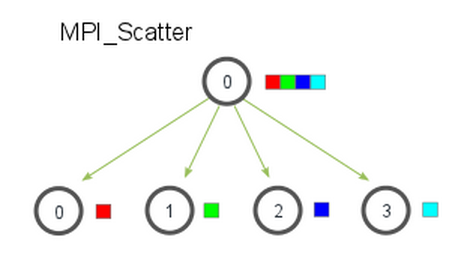
\includegraphics[width=0.4\textwidth]{figs/MPI_Scatter.png}
    \caption{Initial Assembly Result}
\end{figure}

\item During the calculation of the whole graph, Ranks in the same Column/Row are sharing blocks through 
	  MPI\_Allgather.
\begin{figure}[H]
    \centering
    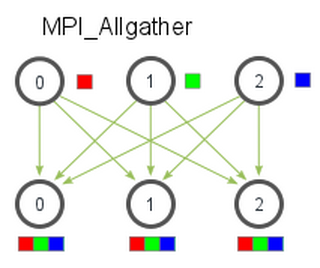
\includegraphics[width=0.3\textwidth]{figs/MPI_Allgather.png}
    \caption{Initial Assembly Result}
\end{figure}

\item To gather the final result to rank 0, MPI\_Scatter method is used.
\begin{figure}[H]
    \centering
    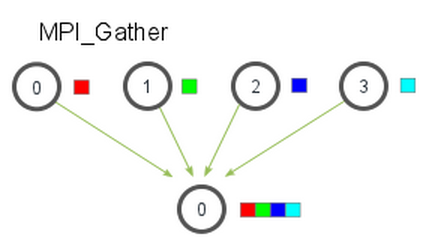
\includegraphics[width=0.4\textwidth]{figs/MPI_Gather.png}
    \caption{Initial Assembly Result}
    \label{initial_profile_result_1}
\end{figure}

\end{enumerate}


